\section{Additional Details on the Experiments in Section~\ref{sec:experiment}}
\label{secapp:experiments}
This section provides datasets, models, and training details for experiments in Section~\ref{sec:experiment}. 
% The code to reproduce our experimental results is included in our Supplementary Material submission.
\subsection{Image Classification on Imagenet}
\textbf{Datasets and Metrics.} The ImageNet dataset, as described in~\cite{deng2009imagenet, russakovsky2015imagenet}, consists of $1.28$ million images for training and $50,000$ images for validation, covering the classification of 1000 different categories. Performance evaluation is based on top-1 and top-5 accuracies. \\\\
\textbf{Models and Baselines.} Our baseline model is the DeiT-tiny model~\cite{touvron2020deit}, which consists of 12 transformer layers, 3 attention heads per layer, and a model dimension of 192. For model setting and setting and configuration, we follow~\cite{touvron2020deit}. Their implementation is available at \href{https://github.com/facebookresearch/deit}{https://github.com/facebookresearch/deit}. The $\lambda_P, \lambda_I, \lambda_D$, and $\beta$ used for our PID DeiT method is $0.8, 0.5, 0.05$, and $0.1$, respectively.
\subsection{Image Segmentation on ADK20 dataset}
\textbf{Datasets and Metrics.} 
The ADE20K dataset is renowned for its incorporation of complex scenes featuring detailed labels, establishing it as one of the most rigorous semantic segmentation datasets. It comprises a training set of $20,210$ images covering 150 semantic classes. Furthermore, the dataset includes $2,000$ images in the validation set and $3,352$ images in the test set. Performance in this task is evaluated using the Single-scale mean Intersection over Union (SS mIoU) and Multi-scale (MS mIoU) metrics.

\textbf{Models and baselines.}
The training configuration and setting for our models are followed by~\cite{strudel2021segmenter}. The baseline model is finetuned with the pretrained DeiT-tiny backbone while our segmenter model used the pretrained PID DeiT-tiny, with $\lambda_P, \lambda_I, \lambda_D$, and $\beta$ are $0.5, 0.3, 0.05$, and $1$, respectively.
\subsection{Language Modeling on WikiText-103}
\textbf{Datasets and Metrics.} 
The WikiText-103 dataset is composed of Wikipedia articles tailored to capture extensive contextual dependencies. Its training set includes roughly $28,000$ articles, totaling around 103 million words. Each article consists of text blocks averaging about $3,600$ words. The validation and test sets contain $218,000$ and $246,000$ words, respectively, divided into 60 articles per set and approximately $268,000$ words each. Our experiment adheres to the standard setup outlined in~\cite{DBLP:conf/iclr/MerityX0S17, schlag2021linear}, which entails segmenting the training data into independent long segments of length $L$ words. For evaluation, we utilize a batch size of $1$ and process the text sequence using a sliding window of size $L$. When calculating perplexity (PPL), we only consider the last position, except for the first segment where all positions are evaluated, consistent with the methodology in~\cite{al2019character, schlag2021linear}.

\textbf{Models and baselines.} For our language modeling implementation, we rely on the publicly available code \textcolor{blue}{\href{https://github.com/IDSIA/lmtool-fwp}{https://github.com/IDSIA/lmtool-fwp}} developed by~\cite{schlag2021linear}. In our experiments, we set the dimensions of keys, values, and queries to 128, while the training and evaluation context length is set to 256. In this experiment, $\lambda_P, \lambda_I, \lambda_D$, and $\beta$ being set to $0.4, 0.5, 0.1$ and $0.3$, respectively, yields the best performance of PIDformer language model.
\subsection{Adversarial Examples and  Out-of-distribution datasets}
\textbf{Imagenet-C} To assess robustness against typical image corruptions, we employ the ImageNet-C dataset~\cite{hendrycks2019benchmarking}, which comprises 15 categories of artificially generated corruptions spanning five levels of severity. ImageNet-C evaluates models using the mean corruption error (mCE) metric, where a lower mCE value indicates greater resilience to corruption.

\textbf{Imagenet-A} ImageNet-A~\cite{hendrycks2021natural} is a dataset consisting of authentic images that have been filtered to deceive ImageNet classifiers. Specifically, it focuses on a subset of 200 classes chosen from the original 1000 classes in ImageNet-1K. Errors made within these 200 classes are regarded as significant, encompassing a wide range of categories represented in ImageNet-1K.

\textbf{Imagenet-O} This dataset comprises examples that have been adversarially filtered to challenge out-of-distribution detectors for ImageNet~\cite{hendrycks2021natural}. It includes samples from the larger ImageNet-22K dataset but excludes those from ImageNet1K. Specifically, samples are chosen if they are confidently misclassified as an ImageNet-1K class by a ResNet-50 model. The evaluation metric utilized is the area under the precision-recall curve (AUPR).

\textbf{Imagenet-R} This dataset comprises diverse artistic interpretations of object classes found in the original ImageNet dataset, a practice discouraged by the creators of the original ImageNet~\cite{hendrycks2021many}. ImageNet-R encompasses 30,000 renditions of images representing 200 classes from the ImageNet dataset, with a selection made from a subset of the ImageNet-1K classes.
\subsection{Adversarial Attacks}
We employ fast gradient sign method (FGSM)~\cite{dong2020benchmarking}, projected gradient descent method (PGD)~\cite{tramer2019adversarial}; and Sparse $L_1$ descent method as well as noise-adding attack
These attacks were
applied to the entire validation set of ImageNet. FGSM and PGD attacks distort the input image with a perturbation budget $\epsilon= 3/255$, and $\epsilon=0.1$ for SPSA, under $l_{\infty}$ norm, while the PGD attack uses 20 steps with a step size of $\alpha = 0.15$. For the SLD and noise attack, we follow the same setting in~\href{https://github.com/cleverhans-lab}{https://github.com/cleverhans-lab}
\subsection{Rank-collapse Analysis}
\label{secapp:cossim}
The average cosine similarity between all pairs of token's representations $(\bx_i, \bx_j)$ in a sequence is computed as
\begin{align}
\nonumber
\frac{1}{N(N - 1)}\sum_{i \neq j}\frac{\bx_i^T\bx_j}{\| \bx_i\|_2\| \bx_j\|_2}.
\end{align} 
% \vspace{-0.15in}
The result is then averaged over 1000 randomly chosen test data in ImageNet. The result is then reported for each layer, as in Fig.~\ref{fig:pid-cossim}.
\section{Technical Proofs}
\subsection{Solution of the first order ODE}
\label{secapp:first-order-ode}
Given $\bm{Q} \in \mathbb{R}^{n \times n}$, $\bm{Y}(t) \in \mathbb{R}^{N \times P}, t > 0$, we are interested in the solution of the first order ODE stated as:
\begin{align}
\label{eq:ode}
    \bm{Y}'(t) = \bm{Q}\bm{Y}(t), \bm{Y}(0) = \bm{Y}^0.
\end{align}
The general solution of~(\ref{eq:ode}) is $\bm{Y}(t) = \mathrm{exp}(\bm{Q}t)\bm{C}$, where $\bm{C} \in \mathbb{R}^{n \times p}$ is an any constant matrix. Indeed, 
\begin{equation}
    \begin{aligned}
        \bm{Y}'(t) &= (\bm{I} + \bm{Q}t + \frac{\bm{Q}^2t^2}{2!} + \frac{\bm{Q}^3t^3}{3!} + \dots)'\bm{C}\\
        &= (\bm{Q} + \bm{Q}^2t + \frac{\bm{Q}^3t}{2!} + \dots)\bm{C}\\
        & = \bm{Q}\mathrm{exp}(\bm{Q}t)\bm{C} = \bm{Q}\bm{Y}(t).
    \end{aligned}
\end{equation}\\\\
To satisfy the intitial condition, $\bm{Y}(0) = \bm{Q}\mathrm{exp}(\bm{Q}0)\bm{C} = \bm{Y}^0$. Hence, $\bm{C} = \bm{Y}^0$ and the solution for the intial value problem in~(\ref{eq:ode}) is $\mathrm{exp}(\bm{Q}t)\bm{Y}^0$.
\\  \\
Every square matrix can be Jordan decomposed as the form of $\bm{Q} = \bm{S}\bm{J}\bm{S}^{-1}$, where $\bm{S}$ is invertible and contains the generalized eigenvectors of $\bm{Q}$, and $\bm{J} = \bm{\mathrm{diag}}(\bm{J}_{\eta_1, m_1}, \bm{J}_{\eta_2, m_2}, \dots, \bm{J}_{\eta_M, m_M}) $ is the Jordan form of matrix $\bm{Q}$ with,\\
$\bm{J}_{\eta_i, m_i} = \begin{bmatrix} 
    \eta_i &  1& \dots &0\\
   \vdots & \ddots & & \vdots\\
    &  & \eta_i& 1\\
    0 & \dots    &   & \eta_i
    \end{bmatrix} \in \mathbb{R}^{m_i \times m_i}$, for $i = 1, \dots, M$ are Jordan blocks and $\eta_1, \dots \eta_M$ are eigenvalues of $\bm{Q}$.
\\
We rewrite the solution of~(\ref{eq:ode}) using the Jordan decomposition as
\begin{equation}
\label{eq:ode-sol}
    \begin{aligned}
        \bm{Y}(t) &= \mathrm{exp}(\bm{Q}t)\bm{Y}^0 = \mathrm{exp}(\bm{S}\bm{J}\bm{S}^{-1}t)\bm{Y}^0\\
        & = (\bm{S}\bm{S}^{-1} + \bm{S}\bm{J}\bm{S}^{-1}t + \frac{(\bm{S}\bm{J}\bm{S}^{-1})^2t^2}{2!} + \dots)\bm{Y}^0\\
        & = \bm{S}\mathrm{exp}(\bm{J}t)\bm{S}^{-1}\bm{Y}^0.
    \end{aligned}
\end{equation}
\\
We are now interested in the asymptotic behavior of the solution in~(\ref{eq:ode-sol}) as $t \rightarrow \infty$.\\
\textit{\textbf{When $\bm{Q}$ only has eigenvalues negative real parts}}. As $\eta_1, \dots \eta_M < 0$, we consider
\begin{equation}
    \begin{aligned}
        \mathrm{exp}(\bm{J}_{\eta_i, m_i}t) &= \sum_{k = 0}^{\infty}\frac{(\bm{J}_{\eta_i, m_i}t)^k}{k!}\\
        & = \begin{bmatrix}
            \displaystyle \sum_{k = 0}^{\infty} \frac{t^k\eta_i^{k}}{k!} & \displaystyle \sum_{k = 1}^{\infty} \frac{t^k\eta_i^{k - 1}}{(k - 1)!} & \dots & \displaystyle \sum_{k = m_i}^{\infty} \frac{t^k\eta_i^{k - m_i + 1}}{(k - m_i + 1)!}\\
            \vdots & \ddots & & &\\
            0&\dots & \displaystyle \sum_{k = 0}^{\infty} \frac{t^k\eta_i^{k}}{k!} & \displaystyle \sum_{k = 1}^{\infty} \frac{t^k\eta_i^{k - 1}}{(k - 1)!}\\
            0& \dots & 0 & \displaystyle \sum_{k = 0}^{\infty} \frac{t^k\eta_i^{k}}{k!}
        \end{bmatrix}\\
        &= \begin{bmatrix}
            e^{\eta_it} & te^{\eta_it} & \dots & t^{m_i - 1}e^{\eta_it}\\
            \vdots & \ddots & & &\\
            0&\dots & e^{\eta_it} & te^{\eta_it}\\
            0& \dots & 0 & e^{\eta_it}
        \end{bmatrix}\\
    \end{aligned}
\end{equation}
which is derived from the result $\bm{J}^k_{\eta_i, m_i} = \begin{bmatrix}
             \eta_i^{k} & \begin{pmatrix} j\\1 \end{pmatrix}\eta_i^{k - 1} & \dots & \begin{pmatrix} j\\m_i - 1 \end{pmatrix}\eta_i^{k - m_i + 1}\\
            \vdots & \ddots & & &\\
            0&\dots & \eta_i^{k} & \begin{pmatrix} j\\1 \end{pmatrix}\eta_i^{k - 1}\\
            0& \dots & 0 & \eta_i^{k}
    \end{bmatrix}\\$  
    % (See~\ref{} )
Therefore, when $t \rightarrow 0, \mathrm{exp}(\bm{J}_{\eta_i, m_i}t)\rightarrow \bm{0}$, making $\mathrm{exp}(\bm{J}t) \rightarrow \bm{0}$ and hence the solution in~(\ref{eq:ode-sol}) will goes to $\bm{0}$ or being stable.\\
\textit{\textbf{When $\bm{Q}$ only has at least one eigenvalue with positive real part}}. Without the loss of generalization, let $\mathrm{Re}(\eta_1) > 0$. Hence $\| \mathrm{exp}(\bm{J}_{\eta_1, m_i}t) \| \rightarrow \infty$ when $t \rightarrow \infty$. In other words, the solution of~(\ref{eq:ode}) will explode or unstable.
% \textit{\textbf{When $\bm{Q}$ some 0 eigenvalues while the rest are negative.}}
\subsection{Proof of Lemma~\ref{lem:state-space-sol}}
\label{secapp:state-space-sol}
The proof of Lemma~\ref{lem:state-space-sol} is the direct result in Appendix~\ref{secapp:first-order-ode}. The solution of the ordinary differential equation (ODE) in~(\ref{eq:ode1}) is
        $\bV(t) = \bm{P}\mathrm{exp}(\bm{J}t)\bm{P}^{-1}\bV^0$,
where $\bm{P}\bm{J}\bm{P}^{-1}$ if the Jordan decomposition of $\bm{K} - \bm{I}$, $\bm{J} = \bm{\mathrm{diag}}(\bm{J}_{\alpha_1, m_1}, \bm{J}_{\alpha_2, m_2}, \dots, \bm{J}_{\alpha_M, m_M})$ and $\alpha_1 \geq \alpha_2 \geq \dots, \geq \alpha_M, M \leq N$ are  eigenvalues $\bK - \bI$. Consequently, we have proved the Lemma~\ref{lem:state-space-sol}
\subsection{Proof of Lemma~\ref{lem:steady-state-state-space-sol}}
\label{secapp:steady-state-state-space-sol}
In Section~\ref{subsec:state-space-analysis}, we have shown that $\bm{K} - \bm{I}$ has a unique largest eigenvalue $\lambda_1 = 0$. This means that the Jordan blocks corresponding with other eigenvalues which has negative real parts will approach $\mathrm{exp}(\bm{J}_{\eta_i, m_i}t) \rightarrow \bm{0}$, for $i = 1, \dots, M;, i \neq 1$, as $t \rightarrow \infty$. As the consequence, $\mathrm{exp}(\bm{J}t)$ are fill with 0 for all entries except for the first entry $\mathrm{exp}(\bm{J}t)(0, 0) = 1$. Hence, the solution in~(\ref{eq:state-space-sol}) becomes 
\begin{align}
\nonumber
    \begin{bmatrix} \displaystyle c_{1,1}\bm{p_1}, & \dots ,& \displaystyle c_{1, D_x}\bm{p_1} \end{bmatrix}.
\end{align}
% Rewriting the initial condition $\bm{Y}^0$ as a decomposition of the generalized eigenvectors $\bm{p}_n$ for $n = 1, \dots, N$ of $\bm{Q}$
% \begin{equation}
%     \begin{aligned}
%         \bm{Y}^0 = \begin{bmatrix}
%             \displaystyle \sum_{n = 1}^{N}c_{1, n}\bm{p}_n & \dots & \displaystyle \sum_{n = 1}^{N}c_{N, n}\bm{p}_n
%         \end{bmatrix}
%     \end{aligned}
% \end{equation}
This concludes the proof.
\subsection{Proof of Lemma~\ref{lem:breg-iter}}
\label{secapp:breg-iter}
For $\bv^{\ell + 1}$ to be the solution of the optimization problem in~(\ref{eqn:breg-op}), since $\bm{0} \in \partial J(\bv^{\ell + 1}) - \bm{p}^{\ell} + \partial G(\bv^{\ell + 1}, \bff)$, hence the iteration becomes:
\begin{equation}
\nonumber
\begin{cases} 
& \bv^{\ell + 1} = \displaystyle \argmin_{\bv} J(\bv) - <\bm{p}^{\ell}, \bv> + G(\bv, \bff) \\
& \bm{p}^{\ell + 1} \in \bm{p}^{\ell} - \partial G(\bv^{\ell + 1}, \bff). 
\end{cases}
\end{equation}
When $G(\bv, \bff) = \frac{\lambda}{2}  \int_{\Omega} \|\bv(x) - \bff(x)\|_2^2 dx$,
\begin{equation}
\nonumber
\begin{aligned}
G(\bv, \bff) - \langle\bm{p}^{\ell}, \bv\rangle &= \frac{\lambda}{2} \int_{\Omega}\Bigg(  \left(  \|\bv(x)\|_2^2 -2\langle\bv(x), \bff(x)\rangle + \|\ \bff(x)\|_2^2 \right ) + \lambda\langle\sum^{\ell}_{m = 1} \left(\bv^m(x) - \bff(x) \right), \bv(x)\rangle \Bigg) dx \\
&= \frac{\lambda}{2} \int_{\Omega} \Bigg( \|\bv(x)\|_2^2 - \lambda\langle\bff(x) - \sum^{\ell}_{m = 1}\Big( \bv^m(x) - \bff(x) \Big), \bv(x)\rangle\Bigg) dx + \text{constant}\\
&= \frac{\lambda}{2} \int_{\Omega} \|\bv(x) - \bff^{\ell}(x)\|_2^2 dx + \text{constant},
\end{aligned}
\end{equation}
where $\bff^{\ell}(x) = \bff^{\ell - 1}(x) + \bff(x) - \bv^{\ell}(x)$. \\
Substituting $G(\bv, \bff) - \langle\bm{p}^{\ell}, \bv\rangle$ into the iteration, it becomes
\begin{equation}
\begin{cases}
   & \bv^{\ell + 1} = \displaystyle \argmin_{\bv} J(\bv) + \frac{\lambda}{2} \int_{\Omega} \|\bv(x) - \bff^{\ell}(x)\|_2^2 dx \\
 & \bff^{\ell}(x) = \bff^{\ell - 1}(x) + \bff(x) - \bv^{\ell}(x).
    \end{cases}
\end{equation}
The iteration in Lemma~\ref{lem:breg-iter} can be reformulated as:
\begin{equation}
\nonumber
   \bv^{\ell + 1} = \displaystyle \argmin_{\bv} J(\bv) + \frac{\lambda}{2} \int_{\Omega} \|\bv(x) - \bff(x) - \bm{e}_{\mathrm{a}}^{\ell}(x)\|_2^2 dx \\
\end{equation}
where $\bm{e}^{\ell}_{\mathrm{a}}(x)= \sum_{m = 1}^{\ell} \bm{e}^m(x) = \sum_{m = 1}^{\ell}\big( \bff(x) - \bv^m(x) \big)$
we conclude the proof for Lemma~\ref{lem:breg-iter}.
% Let $\bv(x, 0) = \bv^{\ell}(x)$ and $\Delta t(x):= \displaystyle \frac{1}{\int_{\Omega}\bigl(k(x, y) + k(y,x)\bigl)dy}$, $\tilde\lambda = \displaystyle \frac{\lambda}{\Delta t}$, the update step at layer $l + 1$ becomes
% \begin{equation}
%     \bv^{\ell + 1}(i) = \sum_{j=1}^N{\rm softmax}\Big({\bq^{\ell}}(i)^\top{\bk^{\ell}}(j)/\sqrt{D_{qk}}\Big){\bv^{\ell}}(j) + \tilde\lambda(\bff(i) - \bv^{\ell}(i)) + \sum_{k = 1}^{\ell} \bigl(\bff(i) - \bv^k(j) \bigl)
% \end{equation}
\subsection{Proof of Lemma~\ref{lem:state-space-P-sol}}
\label{secapp:state-space-P-sol}
To find the solution of Eqn~\ref{eq:odeP}, firstly, we find the solution for the homogenous ODE:
\begin{align}
    \bV^{(h)}{'}(t) = \bigl(\bK - (\lambda_P + 1)\bm{I} \bigl)\bV^{(h)}(t)
\end{align}
From the result in Appendix~\ref{secapp:first-order-ode}, the solution for this ODE is $\mathrm{exp}(\bm{B}t)\bm{C}$ where $\bm{B} = \bK - (\lambda_P + 1)\bm{I}$ and $\bm{C} \in \mathbb{R}^{N \times D_x} $ is any constant matrix.
Secondly, we find a particular solution for~(\ref{eq:odeP}) by solving $\bV^{(p)}{'}(t) = \bm{B}\bV(t)^{(p)} + \lambda_P\bm{F} = \bm{0}$. Since $\bm{B}$ is invertible, the solution for this equation is $\bV^{(p)}(t) = -\lambda_P\bm{B}^{-1}\bm{F}$. It is easy to check that $\bV(t) = \bV^{(h)}(t) + \bV^{(p)}(t)$ is the solution of the $\bV'(t) = \bm{B}\bV(t) + \lambda_P\bm{F}$. Applying the initial condition, $\bV(0) = \bm{C} -\lambda_P\bm{B}^{-1}\bm{F} = \bV^0$, we find $\bm{C} = \bV^0 + \lambda_P\bm{B}^{-1}\bm{F}$. Therefore, we have proved that the solution for the IVP problem in~(\ref{eq:odeP}) is indeed $\bV(t) = \mathrm{exp}(\bm{B}t)(\bV^0 + \bm{B}^{-1}\bm{F}) - \lambda_P\bm{B}^{-1}\bm{F}.$\\ \\
In Section~\ref{subsec:PD-robust}, we show that $\bm{B}$ has only eigenvalues with negative real parts. As the result in Appendix~\ref{secapp:first-order-ode}, when $t \rightarrow 0$, the $\mathrm{exp}(\bm{B}t) \rightarrow \bm{0}$ , leading to the vanishing of the $\bV^{(h)}(t)$. Hence the steady state solution for the ODE in~(\ref{eq:odeP}) becomes $ - \lambda_P\bm{B}^{-1}\bm{F}$.
\\ \\
This concludes the proof.
\subsection{Proof of Proposition~\ref{lem:lambda_P}}
\label{secapp:lambda_P}
We first show that $\bm{B}$ is a strictly diagonal dominant (SDD) matrix, i.e., $|\bm{B}(i, i)| > |\sum_{j \neq i}^N\bm{B}(i, j)|$, for $i, j = 1, \dots, N$. In fact, $|\bm{B}(i, i)| = |\bm{K}(i, i) - \lambda_p - 1| > |1 - \bm{K}(i, i)| = |\sum_{j \neq i}^N\bm{K}(i, j)| = |\sum_{j \neq i}^N\bm{B}(i, j)|$ because $\bm{K}$ is a right-stochastic matrix with all entries in $(0, 1]$ and sum of each row is 1.
\\
Hence, following~\cite{MORACA2007666}, the upper bound of $\| \bm{B}^{-1}\|_{\infty}$, when $\bm{B}$ is an SDD matrix, is given as
\begin{align}
    \| \bm{B}^{-1}\|_{\infty} &\leq \frac{1}{ \displaystyle \min_{i \in N}(|\bm{B}(i, i)| - |\sum_{j \neq i}^N\bm{B}(i, j)|)} \\
    & = \frac{1}{|\bm{K}(i, i) - \lambda_p - 1| - |1 - \bm{K}(i, i)|} = \frac{1}{\lambda_P},
\end{align} where $\displaystyle \| \bm{B}^{-1}\|_{\infty} = \max_{i = 1}^N \sum_{j = 1}^N |\bm{B}^{-1}(i, j)|$.\\
On the other hand, 
\begin{equation}
    \begin{aligned}
    \|-\lambda_P\beta \bm{B}^{-1}\bm{\epsilon}\|_{\infty} &\leq \lambda_P\beta \| \bm{B}^{-1}\|_{\infty}\| \bm{\epsilon}\|_{\infty} \\
    &= \lambda_P \beta \frac{1}{\lambda_P} \bar{\epsilon}
    =\beta\bar{\epsilon}
    \end{aligned}
\end{equation}
For the bounded error get arbitrarily small, we constraint $\beta\bar{\epsilon} \leq \delta$, making $\beta \leq \frac{\delta}{\bar{\epsilon}}$.\\
Here in the proof, we used the submultiplicity property of $\|.\|_{\infty}$ norm of matrices, which is proved as follow:
\begin{equation}
    \begin{aligned}
        \nonumber
        \| \bm{B}^{-1}\bm{\epsilon}\|_{\infty} = \sup_{\bx}\frac{\|\bm{B}^{-1}\bm{\epsilon} \bx\|_{\infty}}{\| \bx\|_{\infty}} &= \sup_{\bx}\frac{\|\bm{B}^{-1}\bm{\epsilon} \bx\|_{\infty} \|\bm{\epsilon} \bx\|_{\infty}}{\|\bm{\epsilon} \bx\|_{\infty}\| \bx\|_{\infty}}\\
        &\leq \sup_{\bx}\frac{\|\bm{B}^{-1}\bm{\epsilon} \bx\|_{\infty}}{\| \bm{\epsilon} \bx\|_{\infty}} \sup_{\bx}\frac{\|\bm{\epsilon} \bx\|_{\infty}}{\| \bx\|_{\infty}}\\
        & \leq \sup_{\bx}\frac{\|\bm{ B^{-1}} \bx\|_{\infty}}{\| \bx\|_{\infty}}\sup_{\bx}\frac{\|\bm{\epsilon} \bx\|_{\infty}}{\| \bx\|_{\infty}}\\
        &= \|\bm{B}^{-1}\|_{\infty}\|\bm{\epsilon}\|_{\infty}
    \end{aligned}
\end{equation}
With this, we conclude the proof of Proposition~\ref{lem:lambda_P}
\subsection{Proof of Lemma~\ref{lem:state-space-PD-sol}}
\label{secapp:state-space-PD-sol}
To find the solution of~(\ref{eq:odePD}), firstly, we find the solution for the homogenous ODE:
\begin{align}
\nonumber
    \bV^{(h)}{'}(t) = \frac{1}{1 + \lambda_D}\bigl(\bK - (\lambda_P + 1)\bm{I} \bigl)\bV^{(h)}(t)
\end{align}
From the result in Appendix~\ref{secapp:first-order-ode}, the solution for this ODE is $\mathrm{exp}(\displaystyle \frac{1}{\lambda_D + 1}\bm{B}t)\bm{C}$ where $\bm{B} = \bK - (\lambda_P + 1)\bm{I}$ and $\bm{C} \in \mathbb{R}^{N \times D_x} $ is any constant matrix.
Secondly, we find a particular solution for~(\ref{eq:odePD}) by solving $\bV^{(p)}{'}(t) = \displaystyle \frac{1}{\lambda_D + 1}(\bm{B}\bV(t)^{(p)} + \lambda_P\bm{F}) = \bm{0}$. Since $\bm{B}$ is invertible, the solution for this equation is $\bV^{(p)}(t) = -\lambda_P\bm{B}^{-1}\bm{F}$. The solution is $\bV(t) = \bV^{(h)}(t) + \bV^{(p)}(t)$. Applying the initial condition, $\bV(0) = \bm{C} -\lambda_P\bm{B}^{-1}\bm{F} = \bV^0$, we find $\bm{C} = \bV^0 + \lambda_P\bm{B}^{-1}\bm{F}$. Therefore, we have proved that the solution for the IVP problem in~(\ref{eq:odePD}) is indeed $\bV(t) = \displaystyle \mathrm{exp}(\frac{1}{\lambda_D + 1}\bm{B}t)(\bV^0 + \bm{B}^{-1}\bm{F}) - \lambda_P\bm{B}^{-1}\bm{F}.$\\ \\
In Section~\ref{subsec:PD-robust}, we show that $\bm{B}$ has only eigenvalues with negative real parts. As the result in Appendix~\ref{secapp:first-order-ode}, when $t \rightarrow 0$, the $\mathrm{exp}(\displaystyle\frac{1}{\lambda_D + 1}\bm{B}t) \rightarrow \bm{0}$ , leading to the vanishing of the $\bV^{(h)}(t)$. Hence the steady state solution for the ODE in~(\ref{eq:odePD}) becomes $ - \lambda_P\bm{B}^{-1}\bm{F}$. We have proved Lemma~\ref{lem:state-space-PD-sol}.
\subsection{Proof of Proposition~\ref{lem:lambda_PI}}
\label{secapp:lambda_PI}
Let
\begin{align}
    \bm{M} = \begin{bmatrix} \bm{0} & \bm{I} \\ \displaystyle -\frac{\lambda_I\bm{I}}{\lambda_D + 1} &\displaystyle \frac{\bm{K} - (\lambda_P + 1)\bm{I}}{\lambda_D + 1} \end{bmatrix}
\end{align}
For the solution of~(\ref{eq:ode-pi}) to be stable, the real part of eigenvalues of $\bm{M}$ must be all negative. Let $\bm{B} := \bm{K} - (\lambda_P + 1)\bm{I}$, for any eigenvalue $\gamma$ of $\bm{M}$
\begin{equation}
\label{eq:det-pi}
\begin{aligned}
\mathrm{det}( \bm{M} - \gamma\bm{I}) &= \mathrm{det}\Bigg( \begin{bmatrix} \bm{-\gamma\bm{I}} & \bm{I} \\ -\displaystyle \frac{\lambda_I}{\lambda_D + 1}\bm{I} & \displaystyle\frac{1}{\lambda_D + 1}(\bm{B} - \gamma\bm{I}) \end{bmatrix}\Bigg) \\
&= \mathrm{det}\Big(\frac{1}{\lambda_D + 1}(-\gamma\bm{B} + \gamma^2\bm{I} + \lambda_I \bm{I})\Big), &&\ (\text{since $\bm{B} - \gamma\bm{I}$ and $-\lambda_I\bm{I}$ are commute, see~\cite{0826aabe-2dc2-393a-bbf2-a98a36b6bed5}}) \\
&= 0\\
% & = (-\gamma)^N\mathrm{det}(\bm{B} - (\gamma + \frac{\lambda_I}{\gamma})\bm{I}) 
\end{aligned}
\end{equation}
Notice that $\gamma = 0$ is not a solution of~(\ref{eq:det-pi}). This fact is proved by contradiction. If $\gamma = 0$ is a solution, $\mathrm{det}(-\gamma\bm{B} + \gamma^2\bm{I} + \lambda_I\bm{I}) = \mathrm{det}(\lambda_I\bm{I}) = (\lambda_I)^N\mathrm{det}(\bm{I}) = (\lambda_I)^N > 0$ because $\lambda_I > 0$. This is contradict to~(\ref{eq:det-pi}). Since $\gamma \neq 0$, we can rewrite~(\ref{eq:det-pi}) as:
\begin{align}
    (-\frac{\gamma}{\lambda_D + 1})^N\mathrm{det}(\bm{B} - (\gamma + \frac{\lambda_I}{\gamma})\bm{I}) &=  0\\
    \iff \mathrm{det}(\bm{B} - (\gamma + \frac{\lambda_I}{\gamma})\bm{I}) &=  0.
\end{align}
Therefore, $\displaystyle \gamma + \frac{\lambda_I}{\gamma}$ are eigenvalues of $\bm{B}$. Given $\kappa_i$, for $i = 1, \dots, m; m \leq N$ are eigenvalues of $\bm{B}$. For each $i$, we find the solution of 
\begin{align}
\label{eq:quad-eigen}
    \gamma_i + \frac{\lambda_I}{\gamma_i} &= \kappa_i\\
    \iff \gamma_i^2 -\kappa \gamma_i + \lambda_I &= 0
\end{align}
Let $\gamma_{i, 1}, \gamma_{i, 1}$ are the solution of~(\ref{eq:quad-eigen}), and then 
\begin{equation}
\label{eq:condition-real}
    \begin{cases}
        \gamma_{i, 1} + \gamma_{i, 2} = \kappa_i\\
        \gamma_{i, 1}\gamma_{i, 2} = \lambda_I
    \end{cases}
    \iff \begin{cases}
        \mathrm{Re}(\gamma_{i, 1}) + \mathrm{Re}(\gamma_{i, 2}) = \mathrm{Re}(\kappa_i)\\
        \mathrm{Im}(\gamma_{i, 1}) + \mathrm{Im}(\gamma_{i, 2}) = \mathrm{Im}(\kappa_i)\\
        \mathrm{Re}(\gamma_{i, 1})\mathrm{Re}(\gamma_{i, 2}) - \mathrm{Im}(\gamma_{i, 1})\mathrm{Im}(\gamma_{i, 2}) = \lambda_I\\
        \mathrm{Re}(\gamma_{i, 1})\mathrm{Im}(\gamma_{i, 2}) + \mathrm{Im}(\gamma_{i, 1})\mathrm{Re}(\gamma_{i, 2}) = 0
    \end{cases}
\end{equation}
In Section~\ref{subsec:PD-robust}, we show that $\bm{B}$ has only eigenvalues with negative real parts. Hence, $\mathrm{Re}(\kappa_i) < 0$. 
Firstly, without any loss of generalization, suppose that $\mathrm{Re}(\gamma_{i, 1}) = 0$. This means
\begin{equation}
    \begin{cases}
        \mathrm{Re}(\gamma_{i, 2}) = \mathrm{Re}(\kappa_i) < 0\\
        - \mathrm{Im}(\gamma_{i, 1})\mathrm{Im}(\gamma_{i, 2}) = \lambda_I\\
        \mathrm{Im}(\gamma_{i, 1})\mathrm{Re}(\gamma_{i, 2}) = 0
    \end{cases}
    \Rightarrow \begin{cases}
        \mathrm{Im}(\gamma_{i, 1}) = 0\\
        - \mathrm{Im}(\gamma_{i, 1})\mathrm{Im}(\gamma_{i, 2}) = 0 \neq \lambda_I > 0
    \end{cases}
\end{equation}
which causes contradiction. Therefore, $\mathrm{Re}(\gamma_{i, 1}) \neq 0$. As the result, $\mathrm{Im}(\gamma_{i, 2}) =\displaystyle -\frac{\mathrm{Im}(\gamma_{i, 1})\mathrm{Re}(\gamma_{i, 2})}{\mathrm{Re}(\gamma_{i, 1})}$, substituting to~(\ref{eq:condition-real}), we obtain
\begin{align}
\label{eq:re1}
    \mathrm{Re}(\gamma_{i, 1})\mathrm{Re}(\gamma_{i, 2}) = \lambda_I - \mathrm{Im}(\gamma_{i, 1})^2\frac{\mathrm{Re}(\gamma_{i, 2})}{\mathrm{Re}(\gamma_{i, 1})}.
\end{align}
Suppose that $\mathrm{Re}(\gamma_{i, 1})\mathrm{Re}(\gamma_{i, 2}) < 0$, hence $\displaystyle \frac{\mathrm{Re}(\gamma_{i, 2})}{\mathrm{Re}(\gamma_{i, 1})} < 0$ leading to $\displaystyle - \mathrm{Im}(\gamma_{i, 1})^2\frac{\mathrm{Re}(\gamma_{i, 2})}{\mathrm{Re}(\gamma_{i, 1})} > 0$, (because $\mathrm{Im}(\gamma_{i, 1})^2 > 0$). Therefore the RHS of~(\ref{eq:re1}) is greater than 0 (since $\lambda_I$ also greater than $0$), which contradicts our assumption that $\mathrm{Re}(\gamma_{i, 1})\mathrm{Re}(\gamma_{i, 2}) < 0$. As a consequence, we obattain the following result:
\begin{equation}
    \begin{cases}
        \mathrm{Re}(\gamma_{i, 1}) + \mathrm{Re}(\gamma_{i, 2}) = \mathrm{Re}(\kappa_i) < 0\\
        \mathrm{Re}(\gamma_{i, 1})\mathrm{Re}(\gamma_{i, 2}) > 0
    \end{cases}
    \iff \begin{cases}
        \mathrm{Re}(\gamma_{i, 1}) < 0\\
        \mathrm{Re}(\gamma_{i, 2}) < 0,
    \end{cases}
\end{equation}
for $i = 1, \dots, m$. Therefore, all eigenvalues of $\bm{M}$ as negative real parts. Combined with result in Appendix~\ref{secapp:first-order-ode}, we have the system described by~(\ref{eq:ode-pi}) has stable solution when $t \rightarrow 0$, for all $\lambda_P, \lambda_I, \lambda_D > 0$. This concludes our proof.
\subsection{The Fretchet derivation of the derivative of $J$ w.r.t $v_j$.}
The partial derivative ${\partial J}/{\partial v_j}$, $j = 1, 2, \dots, D$, is defined through its dot product with an arbitrary function $h_j \in L^{2}(\Omega \times [0, \infty))$ as follows

\begin{align}  
    \frac{\partial J}{\partial v_j}\cdot h_j(x, t) &= \frac{d}{d\tau}J(v_j + \tau h_j)\bigl|_{\tau=0} \nonumber \\ 
&= \frac{1}{2} \left(\frac{d}{d\tau}  \int_{\Omega \times \Omega}(v_j(x) - v_j(y) + \tau h_j(x) - \tau h_j(y))^{2} k(x, y)dxdy\right)\biggl|_{\tau=0} \nonumber \\
&= \left(\int_{\Omega \times \Omega}(v_j(x, t) - v_j(y) + \tau h_j(x) - \tau h_j(y, t))(h_j(x) -h_j(y))k(x, y)dxdy\right)\biggl|_{\tau=0} \nonumber \\
&= \int_{\Omega \times \Omega}(v_j(x) - v_j(y))(h_j(x) -h_j(y))k(x, y)dxdy \nonumber \\
&= \int_{\Omega \times \Omega}(v_j(x) - v_j(y))h_j(x)k(x, y)dxdy - \int_{\Omega \times \Omega}(v_j(x) - v_j(y))h_j(y)k(x, y)dxdy \nonumber
% \frac{d}{d\tau} \int_{\Omega \times \Omega} \bigl(u_i(x) - u_i(y) \bigl)\bigl(h_i(x) - h_i(y) \bigl)k(x, y)dxdy.
\end{align}
Applying a change of variables $(x, y) \rightarrow (y, x)$ to the second term of the above integral, we have
\begin{align}  
\frac{\partial J}{\partial v_j} \cdot h_j(x) &= \int_{\Omega \times \Omega}(v_j(x) - v_j(y))h_j(x)k(x, y)dxdy - \int_{\Omega \times \Omega}(v_j(y) - v_j(x))h_j(x, t)k(y, x)dxdy \nonumber \\
&= \int_{\Omega \times \Omega}(v_j(x) - v_j(y)(k(x, y) + k(y, x))dyh_j(x)dx \nonumber
\end{align}
Thus, the Frechet derivative of J with respect to $v_j$ is given by
\begin{align}  
\nonumber
\frac{\partial J}{\partial v_j} 
&= \int_{\Omega}(v_j(x) - v_j(y)(k(x, y) + k(y, x))dy. 
\end{align}
\subsection{The derivation of the gradient flow of $
 E(v, f)$}
\label{secapp:derE}
 Taking the gradient of $E(\bv, \bff)$ with respect to $\bv$, we obtain
\label{secapp:djv}
\begin{align}
\label{eq:devEu}
    \nabla_{\bm{v}}E = \nabla_{\bm{v}}J + 
    \left[\frac{\partial G}{\partial u_1}, \frac{\partial G}{\partial u_2}, \dots, \frac{\partial G}{\partial u_{D}} \right]^T.
\end{align}
The partial derivative ${\partial G}/{\partial v_j}$, $j = 1, 2, \dots, D$, is defined through its dot product with an arbitrary function $h_j \in L^{2}(\Omega)$ as follows
\begin{align}
\frac{\partial G}{\partial v_j}\cdot h_j(x) &= \frac{d}{d\tau}G(v_j + \tau h_j)\bigl|_{\tau=0} \nonumber\\
&= \frac{\lambda}{2} \left(\frac{d}{d\tau} \int_{\Omega} (v_j(x) - f_j(x) + \tau h_j(x))^2 dx \right)\biggl|_{\tau=0}  \nonumber\\
&= \lambda \int_{\Omega} (v_j(x) - f_j(x))h_j(x)  dx  \nonumber.
\end{align}
Thus, the Frechet derivative of F with respect to $v_j$ is given by
\begin{equation}
\label{eq:partial-devFu}
\frac{\partial G}{\partial v_j} = \lambda (v_j(x) - f_j(x))
\end{equation}
Substituting the formula for ${\partial G}/{\partial v_j}$ in~(\ref{eq:partial-devFu}) into~(\ref{eq:devEu}) for $\nabla_{\bv}E(\bv, \bff)$, we obtain the following gradient flow 
\begin{equation}
    \label{eq:gradient-descent-E}
    \frac{d\bm{v}(x,t)}{dt} = -\nabla_{\bm{v}}E(\bv, \bff) = -\nabla_{\bm{v}}J(\bv)(x) + \lambda \bigl(\bff(x) - \bv(x)\bigl).
\end{equation}
\\
This concludes the derivation.
\subsection{The derivation of~(\ref{eq:dis_breg})}
\label{secapp:grad-flow-breg}
Denote $H(\bv, \bff) :=\displaystyle \frac{\lambda}{2} \int_{\Omega} \|\bv(x) - \bff(x) - \bm{e}^{\ell}(x)\|_2^2 dx$. 
 Taking the gradient of $J(\bv) + H(\bv, \bff)$ with respect to $\bv$, we obtain
\begin{align}
\label{eq:devJHu}
    \nabla_{\bm{v}}E = \nabla_{\bm{v}}J + 
    \left[\frac{\partial H}{\partial v_1}, \frac{\partial H}{\partial v_2}, \dots, \frac{\partial H}{\partial v_{D}} \right]^T.
\end{align}
The partial derivative ${\partial H}/{\partial v_j}$, $j = 1, 2, \dots, D$, is defined through its dot product with an arbitrary function $h_j \in L^{2}(\Omega)$ as follows
\begin{align}
\frac{\partial H}{\partial v_j}\cdot h_j(x) &= \frac{d}{d\tau}H(v_j + \tau h_j)\bigl|_{\tau=0} \nonumber\\
&= \frac{\lambda}{2} \left(\frac{d}{d\tau} \int_{\Omega} (v_j(x) - f_j(x) - e^{\ell}_j(x) + \tau h_j(x))^2 dx \right)\biggl|_{\tau=0}  \nonumber\\
&= \lambda \int_{\Omega} (v_j(x) - f_j(x) -e^{\ell}_j)h_j(x)  dx  \nonumber.
\end{align}
Thus, the Frechet derivative of F with respect to $v_j$ is given by
\begin{equation}
\label{eq:partial-devHu}
\frac{\partial H}{\partial v_j} = \lambda (v_j(x) - f_j(x) - e^{\ell}_j)
\end{equation}
Substituting the formula for ${\partial H}/{\partial v_j}$ in~(\ref{eq:partial-devHu}) into~(\ref{eq:devJHu}) for $\nabla_{\bv}E(\bv, \bff)$, we obtain the following gradient flow 
at iteration $\ell + 1$ 
\begin{equation}
\begin{aligned}
   \label{eq:grad-flow-breg}
        \displaystyle\frac{d\bv(x, t)}{dt} &= \int_{\Omega} \bigl(\bm{v}(y,t) - \bm{v}(x,t) \bigl)\bigl(k(x, y) + k(y,x)\bigl)dy \\
        &+ \lambda \bigl(\bff(x) - \bv(x, t) + \bm{e}^{\ell}(x)\bigl).
\end{aligned}
\end{equation}
Applying Euler method to discretize~(\ref{eq:grad-flow-breg}) with $\Delta t = 1$ and $\bv(x, 0) = \bv^{\ell}(x)$, we approximate the $\bv^{\ell + 1}$ with one-step gradient descent:
\begin{equation}
\begin{aligned}
\nonumber
   % \label{eq:dis_breg}
   \bv^{\ell + 1}(x) 
   % \approx \bv(x, 1) 
   &= \int_{\Omega} \bigl(\bm{v}^{\ell}(y) - \bm{v}^{\ell}(x) \bigl)\bigl(k(x, y) + k(y,x)\bigl)dy \\
   & + \bv^{\ell}(x) + \lambda \bm{e}^{\ell}(x) + \lambda\bm{e}^{\ell}_{\mathrm{a}}(x).
\end{aligned}
\end{equation}
% in~(\ref{eq:grad-flow-breg})
This concludes the derivation.
\section{Additional Experiment results}
\subsection{PID DeiT and softmax DeiT under escalating perturbation attacks.}
We evaluate PID DeiT and softmax DeiT under FGSM and PGD attack methods with increasing perturbation budgets (see Fig.~\ref{fig:pid-deit-more-attacks}) (scaled by 255). The proposed PID DeiT exhibits stronger defense in both attack methods and various perturbation budgets.
\label{secapp:moreattacks}
\begin{figure}[!t]
\centering
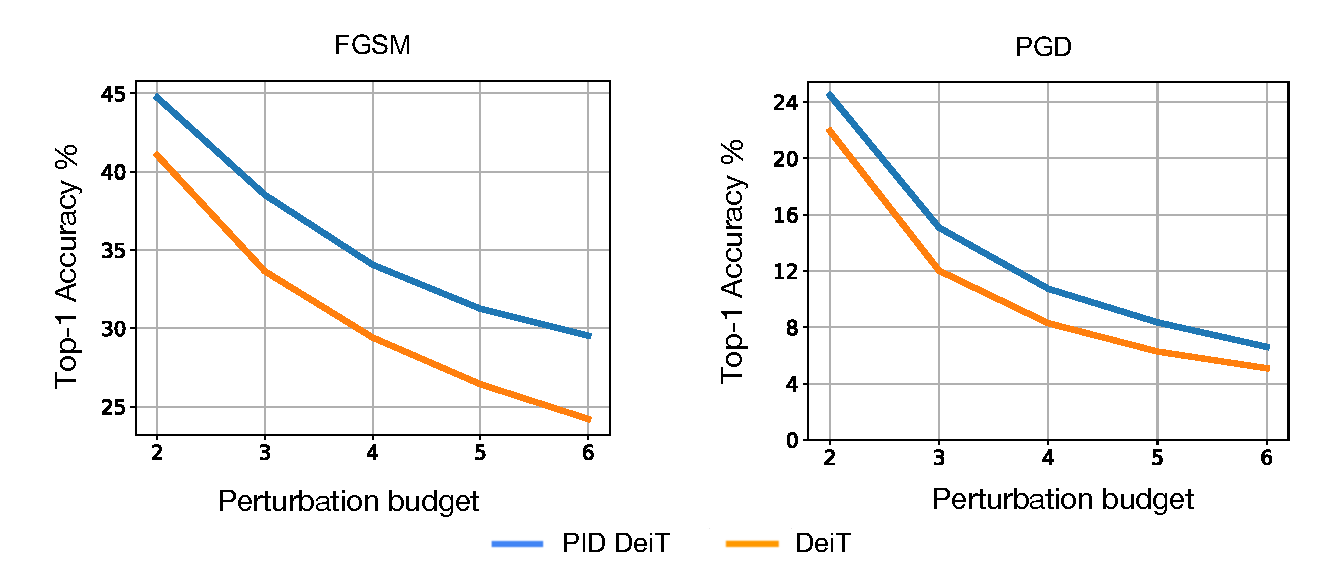
\includegraphics[width=0.9\textwidth]{iclr_2023/pictures/moreattacks.pdf}
% \vspace{-0.3in}
\caption{\small The top-1 classification accuracy curves on ImageNet against FGSM and PGD attack methods, plotted against perturbation budgets (scaled by 255).}
\label{fig:pid-deit-more-attacks} 
% \vspace{-0.in}
\end{figure}
